\documentclass{standalone}
\usepackage{tikz,amsmath}
\usetikzlibrary{decorations.pathmorphing}
\tikzset{block/.style = {draw, fill=white, very thick, rectangle, minimum height=1cm, minimum width=2cm},}
\tikzset{sum/.style= {draw, fill=white, very thick, circle, node distance=1cm},}
\tikzset{nblock/.style = {draw, very thick, rectangle, minimum height=1cm, minimum width=2cm}}
\begin{document}
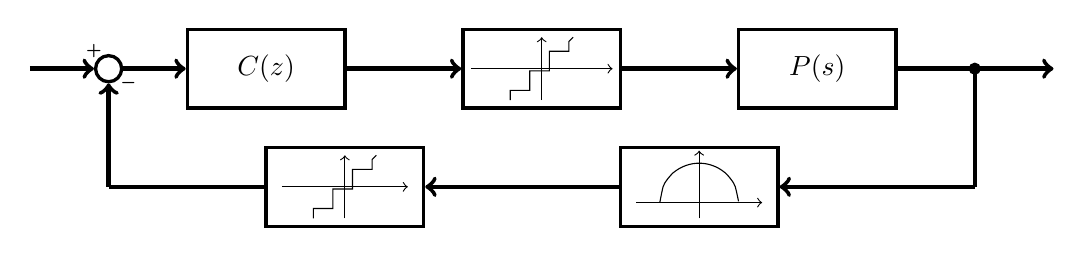
\begin{tikzpicture}[scale=2]
    \node[sum](sum)at(-1,0){};
    \draw[->,ultra thick](-1.5,0)node[above right]{}--(sum.180)node[above]{$\scriptscriptstyle\boldsymbol{+}$};
    \node[block, right of=sum, node distance=2cm](c){$C(z)$};

    \draw[->,ultra thick](sum.0)--(c.180);
    \filldraw[black](4.5,0)circle(1pt);

    \draw[->,ultra thick](4.5,0)--(5,0);
    \draw[-,ultra thick](4.5,-0.75)--(4.5,0);

    \node[nblock]at(1.75,0)(p){};
    \draw[->](1.3,0)--(2.2,0);
    \draw[->](1.75,-0.2)--(1.75,0.2);
    \draw[decorate, decoration=zigzag](1.55,-0.2)--(1.95,0.2);

    \node[block]at(3.5,0)(j){$P(s)$};
    \draw[->,ultra thick](p.0)--(j.180);
    \draw[-,ultra thick](j.0)--(4.5,0);
    \draw[->,ultra thick](c.0)--(p.180);


    \node[nblock]at(0.5,-0.75)(h){};
    \draw[->](0.1,-0.75)--(0.9,-0.75);
    \draw[->](0.5,-0.95)--(0.5,-0.55);
    \draw[decorate, decoration=zigzag](0.3,-0.95)--(0.7,-0.55);

    \node[nblock]at(2.75,-0.75)(z){};
    \draw[->](2.35,-0.85)--(3.15,-0.85);
    \draw[->](2.75,-0.95)--(2.75,-0.52);
    \draw[-]plot[smooth, domain=2.5:3](\x,{-0.85+(0.0625-(\x-2.75)^2)^0.5});
    \draw[->,ultra thick](4.5,-0.75)--(z.0);
    \draw[->,ultra thick](z.180)--(h.0);
    \draw[-,ultra thick](h.180)--(-1,-0.75);

    \draw[->,ultra thick](-1,-0.75)--(sum.270)node[right]{$\scriptscriptstyle\boldsymbol{-}$};
\end{tikzpicture}
\end{document}